\begin{center}
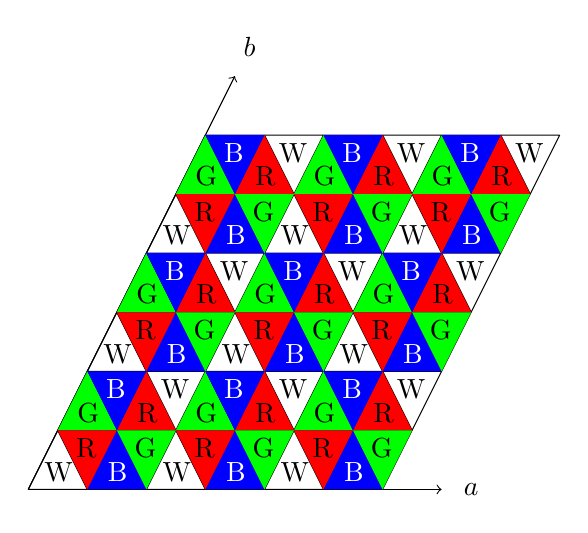
\begin{tikzpicture}[yslant=0, xslant=0.5, scale=0.75]
	\draw (0, 0) grid (6, 6);


	\foreach \x in {1, ..., 6}{
		\draw (\x, 0) -- (0, \x);
	}
	\foreach \x in {1, ..., 5}{
		\draw (\x, 6) -- (6, \x);
	}
	\draw[->] (0, 0) -- (7, 0);
	\node at (7.5, 0) (a) {$a$};

	\draw[->] (0, 0) -- (0, 7);
	\node at (0, 7.5) (b) {$b$};

	\foreach \x in {1, 3, 5}{
		\foreach \y in {1, 3, 5}{	
			\fill[red] (\x, \y) -- (\x + 1, \y) -- (\x, \y + 1) -- cycle;
			\node at (\x+0.365, \y+0.3) (R) {R};
		}
	}
	\foreach \x in {0, 2, 4}{
	    \foreach \y in {0, 2, 4}{
			\node at (\x+0.365, \y+0.3) (W) {W};
		}
	}
	\foreach \x in {1, 3, 5}{
	    \foreach \y in {0, 2, 4}{
			\fill[blue] (\x, \y) -- (\x + 1, \y) -- (\x, \y + 1) -- cycle;
			\node[white] at (\x+0.365, \y+0.3) (B) {B};
		}
	}
	\foreach \x in {0, 2, 4}{
		\foreach \y in {1, 3, 5}{	
			\fill[green] (\x, \y) -- (\x + 1, \y) -- (\x, \y + 1) -- cycle;
			\node at (\x+0.365, \y+0.3) (G) {G};
		}
	}
	\foreach \x in {1, 3, 5}{
		\foreach \y in {1, 3, 5}{	
			\fill[red] (\x, \y) -- (\x - 1, \y) -- (\x, \y - 1) -- cycle;
			\node at (\x-0.365, \y-0.3) (R) {R};
		}
	}
	\foreach \x in {2, 4, 6}{
	    \foreach \y in {2, 4, 6}{
			\node at (\x-0.365, \y-0.3) (W) {W};
		}
	}
	\foreach \x in {1, 3, 5}{
	    \foreach \y in {2, 4, 6}{
			\fill[blue] (\x, \y) -- (\x - 1, \y) -- (\x, \y - 1) -- cycle;
			\node[white] at (\x-0.365, \y-0.3) (B) {B};
		}
	}
	\foreach \x in {2, 4, 6}{
		\foreach \y in {1, 3, 5}{	
			\fill[green] (\x, \y) -- (\x - 1, \y) -- (\x, \y - 1) -- cycle;
			\node at (\x-0.365, \y-0.3) (G) {G};
		}
	}


\end{tikzpicture}
\end{center}